\documentclass[11pt,twoside]{book}

% this requres the installation of texlive-pstricks, as that is needed
% by the vaucanson-g.sty and VCColor-names.def files

\usepackage{palatino}
\usepackage{url}
\usepackage{epsfig}
\usepackage{listings}
\usepackage[table]{xcolor}
\usepackage{wrapfig}
\usepackage{hyperref}

\setlength{\headheight}{0pt}
%\setlength{\footheight}{0pt}
\setlength{\topmargin}{-.5in}
\setlength{\oddsidemargin}{-0.25in}
\setlength{\evensidemargin}{-0.25in}
\setlength{\textwidth}{7truein}
\setlength{\textheight}{9.0truein}
\setlength{\parskip}{6pt}

\newcommand{\und}[1]{\underline{\smash{#1}}}
\newcommand{\leftshift}{<<}

\newenvironment{itemlist}{
\begin{itemize}
\setlength{\itemsep}{0pt}
\setlength{\parskip}{0pt}}
{\end{itemize}}

\newenvironment{numlist}{
\begin{enumerate}
\setlength{\itemsep}{0pt}
\setlength{\parskip}{0pt}}
{\end{enumerate}}

\newcommand{\asminstructionsummary}[7]{
\noindent\begin{tabular}{p{1in}p{#6}p{#7}}
\multicolumn{3}{p{6.7in}}{\bf Instruction: #1} \\
\em Syntax: & \multicolumn{2}{p{5.7in}}{\tt #2} \\
\em Semantics: & \multicolumn{2}{p{5.7in}}{#3} \\
\em Examples: & \tt #4 & \tt #5 \\
\end{tabular}
}

\raggedbottom

\lstset{frameround=fttt,captionpos=b}

\begin{document}

\title {Program and Data Representation}
\author {by Aaron Bloomfield}
\maketitle

\cleardoublepage
\pagenumbering{roman}
\addcontentsline{toc}{part}{Table of Contents}
\tableofcontents

\cleardoublepage
\addcontentsline{toc}{part}{List of Figures}
\listoffigures

\cleardoublepage
\addcontentsline{toc}{part}{List of Tables}
\listoftables

\cleardoublepage
\addcontentsline{toc}{part}{List of Listings}
\lstlistoflistings

\cleardoublepage
\pagenumbering{arabic}

\chapter{Introduction}

\section{Purpose}

\section{How to use this book}

\section{History}



\part{C++}

\chapter{Introduction}

\section{Hello world}

\section{Data types}

\section{Control structures}

\section{Classes and objects}

\section{Header files}



\chapter{Pointers, References, and Memory Management}

\section{Pointers}

\section{Dynamic memory allocation}

\section{References}


\chapter{Arrays}


\chapter{Standard Template Library}

\section{Introduction}

\section{\tt vector}

\section{\tt linked\_list}

\section{\tt string}

\section{\tt \ldots}


\chapter{Advanced C++ Concepts and C++11}

\section{Inheritance}

\section{Dynamic dispatch}

\section{Templates}


\part{Data Structures}

\chapter{Big-Oh Comparisons}

\section{Introduction}

\section{Big-Oh versus Big-Theta versus Big-Omega}

\section{Formal proofs}


\chapter{Lists}

\section{Linked lists}

\section{Stacks}

\section{Queues}


\chapter{Trees}

\section{Binary trees}

\section{Binary search trees}

\section{AVL trees}

\section{Red-black trees}

\section{Splay trees}

\section{Other tree applications}



\chapter{Hashes}

\section{Hash functions}

\section{The hash table}

\section{Collision resolution}

\section{Analysis}


\chapter{Heaps}

\section{Structure property}

\section{Ordering property}

\section{Array storage}

\section{Huffman coding}

\chapter{Graphs}

\section{Introduction}

\section{Representation}

\section{Topological sort}

\section{Traveling salesperson}

\section{Shortest path}

\section{Minimum spanning tree}



\part{Data Representation}

\chapter{Integers}

\section{Sign-and-magnitude}

\section{One's complement}

\section{Two's complement}

\section{BigInteger representation}


\chapter{Floating-point Numbers}

\section{Older representations}

\section{IEEE 754 floating point standard}



\chapter{Strings}

\section{ASCII versus UNICODE}

\section{String representation}


\chapter{Memory}

\section{\ldots}

\part{Assembly and Machine Language}

\chapter{IBCM: The Itty Bitty Computing Machine}
\input{ibcm}


\chapter{32-bit x86 Assembly}

\begin{quotation}
\ldots
\end{quotation}

\noindent {\em This chapter was derived from a document written by Adam Ferrari and later updated by Alan Batson, Mike Lack, Anita
Jones, and Aaron Bloomfield}

\section{Introduction}

This small guide, in combination with the material covered in the
class lectures on assembly language programming, should provide enough
information to do the assembly language labs for this class. In this
guide, we describe the basics of 32-bit x86 assembly language
programming, covering a small but useful subset of the available
instructions and assembler directives. However, real x86 programming
is a large and extremely complex universe, much of which is beyond the
useful scope of this class. For example, there exists real (albeit
older) x86 code running in the world was written using the 16-bit
subset of the x86 instruction set. Using the 16-bit programming model
can be quite complex~-- it has a segmented memory model, more
restrictions on register usage, and so on. In this guide we'll
restrict our attention to the more modern aspects of 32-bit x86
programming, and delve into the instruction set only in enough detail
to get a basic feel for programming x86 compatible chips at the
hardware level.

\section{Registers}

Modern (i.e., 386 and beyond) x86 processors have eight 32-bit general
purpose registers, as depicted in
Figure~\ref{x86-register-diagram.fig}. The register names are mostly
historical in nature. For example, EAX used to be called the
``accumulator'' since it was used by a number of arithmetic
operations, and ECX was known as the ``counter'' since it was used to
hold a loop index. Whereas most of the registers have lost their
special purposes in the modern instruction set, by convention, two are
reserved for special purposes~-- the stack pointer (ESP) and the base
pointer (EBP).

\begin{figure}[h]
\begin{center}
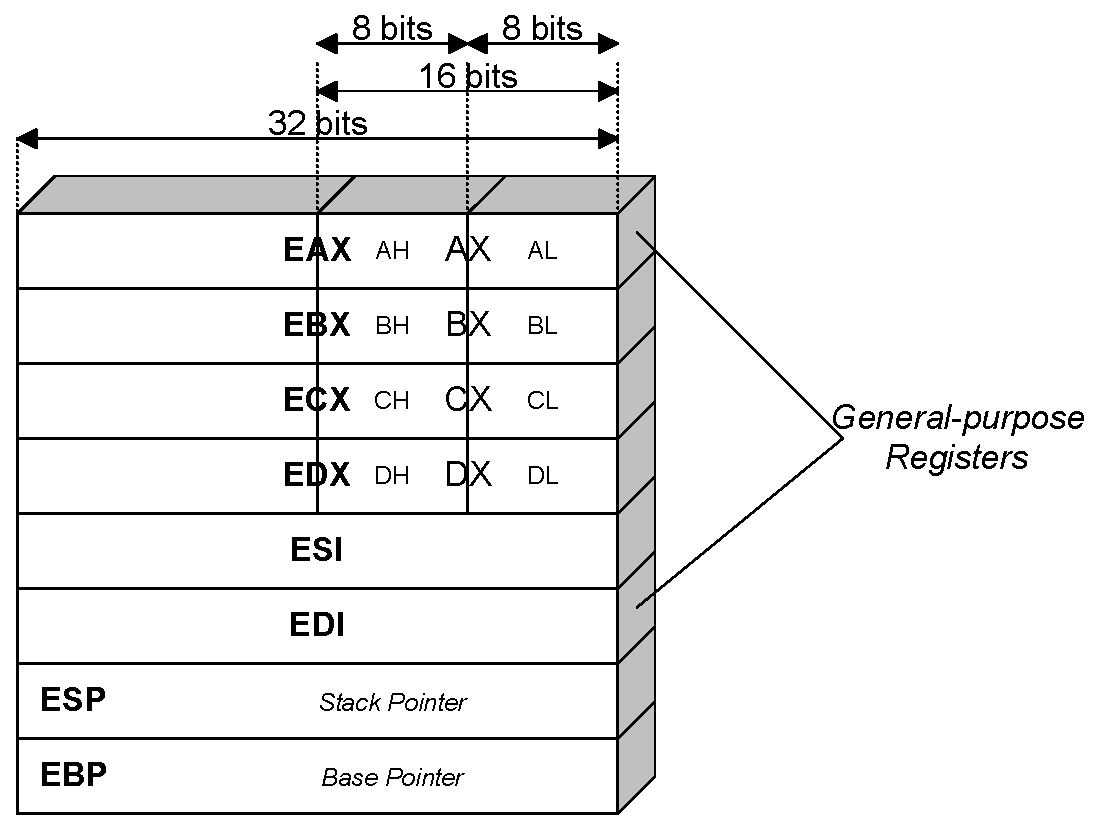
\includegraphics[width=4in]{x86-32bit/x86-register-diagram.pdf}
\end{center}
\caption{The x86 register set}
\label{x86-register-diagram.fig}
\end{figure}

In some cases, namely EAX, EBX, ECX, and EDX, subsections of the
registers may be used.  For example, the least significant 2 bytes of
EAX can be treated as a 16-bit register called AX.  The least
significant byte of AX can be used as a single 8-bit register called
AL, while the most significant byte of AX can be used as a single
8-bit register called AH. It is important to realize that these names
refer to the same physical register. When a two-byte quantity is
placed into DX, the update affects the value of EDX (in particular,
the least significant 16 bits of EDX). These ``sub-registers''
are mainly hold-overs from older, 16-bit versions of the instruction
set. However, they are sometimes convenient when dealing with data
that are smaller than 32-bits (e.g., 1-byte ASCII characters).

When referring to registers in assembly language, the names are not
case-sensitive. For example, the names EAX and eax refer to the same
register.

\section{Memory and Addressing Modes}

\subsection{Declaring Static Data Regions}

You can declare static data regions (analogous to global variables) in
x86 assembly using special assembler directives for this purpose.
Data declarations should be preceded by the .DATA directive. Following
this directive, the directives DB, DW, and DD can be used to declare
one, two, and four byte data locations, respectively. Declared
locations can be labeled with names for later reference - this is
similar to declaring variables by name, but abides by some lower level
rules. For example, locations declared in sequence will be located in
memory next to one another.  Some example declarations are depicted in
Listing~\ref{x86-declaring-memory-regions.lst}.

\begin{figure}[h]
\lstinputlisting[caption=Declaring x86 memory regions,label={x86-declaring-memory-regions.lst},backgroundcolor=\color{white},frame=trBL,linewidth=7in,xleftmargin=0in,language={[x86masm]Assembler}]{x86-32bit/code/memory-regions.s}
\end{figure}

The last example in Listing~\ref{x86-declaring-memory-regions.lst}
illustrates the declaration of an array.  Unlike in high level
languages where arrays can have many dimensions and are accessed by
indices, arrays in assembly language are simply a number of cells
located contiguously in memory. Two other common methods used for
declaring arrays of data are the TIMES directive and the use of string
literals. The TIMES directive tells the assembler to duplicate an
expression a given number of times. For example, the statement ``TIMES
4 DB 2'' is equivalent to ``2, 2, 2, 2''. Some examples of declaring
arrays are depicted in Listing~\ref{x86-declaring-arrays.lst}.

\begin{figure}[h]
\lstinputlisting[caption=Declaring x86 arrays in memory,label={x86-declaring-arrays.lst},backgroundcolor=\color{white},frame=trBL,linewidth=7in,xleftmargin=0in,language={[x86masm]Assembler}]{x86-32bit/code/declaring-arrays.s}
\end{figure}

\subsection{Addressing Memory}
\label{addressing-memory.sec}

Modern x86-compatible processors are capable of addressing up to
$2^{32}$ bytes of memory; that is, memory addresses are 32-bits wide.
For example, in Listings~\ref{x86-declaring-memory-regions.lst} and
\ref{x86-declaring-arrays.lst}, where we used labels to refer to memory
regions, these labels are actually replaced by the assembler with
32-bit quantities that specify addresses in memory. In addition to
supporting referring to memory regions by labels (i.e. constant
values), the x86 provides a flexible scheme for computing and
referring to memory addresses:

{\bf x86 Addressing Mode Rule}~-- Up to two of the 32-bit registers
and a 32-bit signed constant can be added together to compute a memory
address. One of the registers can be optionally pre-multiplied by 2,
4, or 8.

To see this memory addressing rule in action, we'll look at some
example mov instructions.  As we'll see later in
Section~\ref{data-movement-instructions.sec}, the {\tt mov} instruction
moves data between registers and memory.  This instruction has two
operands~-- the first is the destination (where we're moving data {\em
  to}) and the second specifies the source (where we're getting the
data {\em from}). Some examples of mov instructions using address
computations that obey the above rule are shown in
Listing~\ref{x86-valid-addressing-modes.lst}.

\begin{figure}[h]
\lstinputlisting[caption={Valid x86 addressing modes},label={x86-valid-addressing-modes.lst},backgroundcolor=\color{white},frame=trBL,linewidth=7in,xleftmargin=0in,language={[x86masm]Assembler}]{x86-32bit/code/valid-addressing-modes.s}
\end{figure}

Some examples of incorrect address calculations are shown in Listing~\ref{x86-invalid-addressing-modes.lst}.

\begin{figure}[h]
\lstinputlisting[caption={Invalid x86 addressing modes},label={x86-invalid-addressing-modes.lst},backgroundcolor=\color{white},frame=trBL,linewidth=7in,xleftmargin=0in,language={[x86masm]Assembler}]{x86-32bit/code/invalid-addressing-modes.s}
\end{figure}


\subsection{Size Directives}

In general, the intended size of the of the data item at a given memory address can be inferred
from the assembly code instruction in which it is referenced. For example, in all of the above
instructions, the size of the memory regions could be inferred from the size of the register operand~-- when we were loading a 32-bit register, the assembler could infer that the region of memory
we were referring to was 4 bytes wide. When we were storing the value of a one byte register to
memory, the assembler could infer that we wanted the address to refer to a single byte in memory.
However, in some cases the size of a referred-to memory region is ambiguous. Consider the instruction {\tt mov [ebx], 2}.


Should this instruction move the value 2 into the single byte at
address EBX? Perhaps it should move the 32-bit integer representation
of 2 into the 4-bytes starting at address EBX. Since either is a valid
possible interpretation, the assembler must be explicitly directed as
to which is correct.  The size directives {\tt BYTE PTR}, {\tt WORD
  PTR}, and {\tt DWORD PTR} serve this purpose. For examples, see
Listing~\ref{x86-size-directives.lst}.

\begin{figure}[h]
\lstinputlisting[caption={x86 size directive usage},label={x86-size-directives.lst},backgroundcolor=\color{white},frame=trBL,linewidth=7in,xleftmargin=0in,language={[x86masm]Assembler}]{x86-32bit/code/size-directives.s}
\end{figure}


\section{Instructions}

Machine instructions generally fall into three categories: data movement, arithmetic/logic,
and control-flow. In this section, we will look at important examples of x86 instructions from
each category. This section should not be considered an exhaustive list of x86 instructions, but
rather a useful subset.

In this section, we will use the following notation:

\begin{itemlist}
\item $<$reg32$>$ - means any 32-bit register described in Section 2, for example, ESI.
\item $<$reg16$>$ - means any 16-bit register described in Section 2, for example, BX.
\item $<$reg8$>$ - means any 8-bit register described in Section 2, for example AL.
\item $<$reg$>$ - means any of the above.
\item $<$mem$>$ - will refer to a memory address, as described in Section~\ref{addressing-memory.sec}, for example {\tt [EAX]}, or
{\tt [var+4]}, or {\tt DWORD PTR [EAX+EBX]}.
\item $<$con32$>$ - means any 32-bit constant.
\item $<$con16$>$ - means any 16-bit constant.
\item $<$con8$>$ - means any 8-bit constant.
\item $<$con$>$ - means any of the above sized constants.
\end{itemlist}

\subsection{Data Movement Instructions}
\label{data-movement-instructions.sec}

\asminstructionsummary{mov}
{mov $<$reg$>$,$<$reg$>$\newline mov $<$reg$>$,$<$mem$>$\newline mov $<$mem$>$,$<$reg$>$\newline mov $<$reg$>$,$<$const$>$\newline mov $<$mem$>$,$<$const$>$}
{The mov instruction moves the data item referred to by its second
  operand (i.e.  register contents, memory contents, or a constant
  value) into the location referred to by its first operand (i.e. a
  register or memory). While register-to-register moves are possible,
  direct memory-to-memory moves are not. In cases where memory
  transfers are desired, the source memory contents must first be
  loaded into a register, then can be stored to the destination memory
  address.}
{mov eax, ebx \linebreak mov BYTE PTR [var], 5 }
{; transfer ebx to eax\linebreak; store the value 5 into the byte at\linebreak; memory location ``var''}
{2.2in}{3.5in}

\asminstructionsummary{push}
{push $<$reg32$>$\newline push $<$mem$>$\newline push $<$con32$>$}
{The push instruction places its operand onto the top of the hardware supported
stack in memory. Specifically, push first decrements ESP by 4, then places its
operand into the contents of the 32-bit location at address [ESP]. ESP (the stack
pointer) is decremented by push since the x86 stack grows down~-- i.e. the stack
grows from high addresses to lower addresses.}
{push eax\newline push [var]}
{; push the contents of eax onto the stack\newline
; push the 4 bytes at address ``var'' onto stack}
{1in}{4.7in}

\asminstructionsummary{pop}
{pop $<$reg32$>$\newline pop $<$mem$>$}
{The pop instruction removes the 4-byte data element from the top of
  the hardware supported stack into the specified operand (i.e.
  register or memory location). Specifically, pop first moves the 4
  bytes located at memory location [ESP] into the specified register or
  memory location, and then increments SP by 4.}
{pop edi \newline pop [ebx]}
{; pop the top element of the stack into EDI.\newline
; pop the top element of the stack into memory at\newline
; the four bytes starting at location EBX.}
{1in}{4.7in}

\asminstructionsummary{lea}
{lea $<$reg32$>$,$<$mem$>$}
{The lea instruction places the address specified by its second
  operand into the register specified by its first operand. Note, the
  contents of the memory location are not loaded~-- only the effective
  address is computed and placed into the register.  This is useful
  for obtaining a ``pointer'' into a memory region.}
{lea eax, [var]\newline lea edi, [ebx+4*esi]}
{; the address of ``var'' is placed in EAX \newline
; the value EBX+4*ESI is placed in EDI}
{1.85in}{3.85in}

\subsection{Arithmetic and Logic Instructions}

\asminstructionsummary{add, sub}
{add $<$reg$>$,$<$reg$>$ \hspace{0.5in} sub $<$reg$>$,$<$reg$>$ \newline
add $<$reg$>$,$<$mem$>$ \hspace{0.5in} sub $<$reg$>$,$<$mem$>$ \newline
add $<$mem$>$,$<$reg$>$ \hspace{0.5in} sub $<$mem$>$,$<$reg$>$ \newline
add $<$reg$>$,$<$con$>$ \hspace{0.5in} sub $<$reg$>$,$<$con$>$ \newline
add $<$mem$>$,$<$con$>$ \hspace{0.5in} sub $<$mem$>$,$<$con$>$}
{The add instruction adds together its two operands, storing the
  result in its first operand. Similarly, the sub instruction
  subtracts its second operand from its first.  Note, whereas both
  operands may be registers, at most one operand may be a memory
  location.}
{add eax, 10\newline 
sub [var], esi\newline\newline\newline
add BYTE PTR [var], 10}
{; add 10 to the contents of EAX. \newline
; subtract the contents of ESI from \newline
; the 32-bit integer stored at \newline
; memory location ``var''.\newline
; add 10 to the single byte stored\newline
; at memory address ``var''.\newline}
{2.2in}{3.5in}

\asminstructionsummary{inc, dec}
{inc $<$reg$>$ \hspace{0.5in} dec $<$reg$>$\newline
inc $<$mem$>$ \hspace{0.5in} dec $<$mem$>$}
{The inc instruction increments the contents of its operand by one,
  and similarly dec decrements the contents of its operand by one.}
{dec eax \newline inc DWORD PTR [var]}
{; subtract one from the contents of EAX. \newline
; add one to the 32-bit integer stored at \newline
; memory location ``var''.}
{1.8in}{3.9in}

\asminstructionsummary{imul}
{imul $<$reg32$>$,$<$reg32$>$\newline
imul $<$reg32$>$,$<$mem$>$\newline
imul $<$reg32$>$,$<$reg32$>$,$<$con$>$\newline
imul $<$reg32$>$,$<$mem$>$,$<$con$>$}
{The imul instruction has two basic formats: two-operand (first two
syntax listings above) and three-operand (last two syntax listings
above).  The two-operand form multiplies its two operands together and
stores the result in the first operand. The result (i.e., first)
operand must be a register.  The three operand form multiplies its
second and third operands together and stores the result in its first
operand. Again, the result operand must be a register.  Furthermore,
the third operand is restricted to being a constant value.}
{imul eax, [var]\newline\newline\newline
imul esi, edi, 25}
{; multiply the contents of EAX by the \newline
; 32-bit contents of the memory location \newline
; ``var''. Store the result in EAX.\newline
; multiply the contents of EDI by 25. \newline
; Store the result in ESI.}
{1.8in}{3.9in}

\asminstructionsummary{idiv}
{idiv $<$reg32$>$\newline
idiv $<$mem$>$}
{The idiv instruction is used to divide the contents of the 64 bit
  integer EDX:EAX (constructed by viewing EDX as the most significant
  four bytes and EAX as the least significant four bytes) by the
  specified operand value. The quotient result of the division is
  stored into EAX, while the remainder is placed in EDX. This
  instruction must be used with care. Before executing the
  instruction, the appropriate value to be divided must be placed into
  EDX and EAX. Clearly, this value is overwritten when the idiv
  instruction is executed.}
{idiv ebx \newline\newline\newline idiv DWORD PTR [var]}
{; divide the contents of EDX:EAX by the \newline
; contents of EBX. Place the quotient \newline
; in EAX and the remainder in EDX.\newline
; same as above, but divide by the \newline
; 32-bit value stored at memory \newline
; location ``var''.}
{1.9in}{3.8in}

\asminstructionsummary{and, or, xor}
{and $<$reg$>$,$<$reg$>$ \hspace{0.25in} or $<$reg$>$,$<$reg$>$ \hspace{0.25in} xor $<$reg$>$,$<$reg$>$ \newline
and $<$reg$>$,$<$mem$>$ \hspace{0.25in} or $<$reg$>$,$<$mem$>$ \hspace{0.25in} xor $<$reg$>$,$<$mem$>$ \newline
and $<$mem$>$,$<$reg$>$ \hspace{0.25in} or $<$mem$>$,$<$reg$>$ \hspace{0.25in} xor $<$mem$>$,$<$reg$>$ \newline
and $<$reg$>$,$<$con$>$ \hspace{0.25in} or $<$reg$>$,$<$con$>$ \hspace{0.25in} xor $<$reg$>$,$<$con$>$ \newline
and $<$mem$>$,$<$con$>$ \hspace{0.25in} or $<$mem$>$,$<$con$>$ \hspace{0.25in} xor $<$mem$>$,$<$con$>$}
{These instructions perform the specified logical operation (logical
bitwise and, or, and exclusive or, respectively) on their operands,
placing the result in the first operand location.}
{and eax, 0fH \newline xor edx, edx}
{; clear all but the last 4 bits of EAX. \newline ; set the contents of EDX to zero.}
{1.7in}{4in}

\asminstructionsummary{not}
{not $<$reg$>$ \newline not $<$mem$>$}
{Performs the logical negation of the operand contents (i.e., flips all bit values).}
{not BYTE PTR [var]}
{; negate all bits in the byte at the \newline ; memory location ``var''.}
{1.7in}{4in}

\asminstructionsummary{neg}
{neg $<$reg$>$ \newline neg $<$mem$>$}
{Performs the arithmetic (i.e., two's complement) negation of the operand contents.}
{neg eax \newline neg [var]}
{; negate the contents of EAX. \newline ; negate the contests of ``var''}
{1.4in}{4.3in}

\asminstructionsummary{shl, shr}
{shl $<$reg$>$,$<$con8$>$ \hspace{0.5in} shr $<$reg$>$,$<$con8$>$\newline
shl $<$mem$>$,$<$con8$>$ \hspace{0.5in} shr $<$mem$>$,$<$con8$>$\newline
shl $<$reg$>$,cl \hspace{0.92in} shr $<$reg$>$,cl\newline
shl $<$mem$>$,cl \hspace{0.92in} shr $<$mem$>$,cl}
{These instructions shift the bits in their first operand's contents
  left and right ({\tt shl} and {\tt shr}, respectively), padding the
  resulting empty bit positions with zeros. The shifted operand can be
  shifted up to 31 places. The number of bits to shift is specified
  by the second operand, which can be either an 8-bit constant or the
  register CL. In either case, shifts counts of greater then 31 are
  performed modulo 32.}
{shl eax 5 \newline\newline shr [var] 3}{; shift the contents of eax left by 5 bit \newline ; positions \newline ; shift the contents of ``var'' right by 3 \newline ; bit positions}{1.4in}{4.3in}

\subsection{Control Flow Instructions}

In this section, we will refer to labeled locations in the program
text as $<$label$>$. Labels can be inserted anywhere in x86 assembly
code text by entering a label name followed by a colon. For example,
consider the code fragment in Listing~\ref{x86-labeled-code-location.lst}.
The second instruction in this code fragment is labeled ``begin''.
Elsewhere in the code, we can refer to the memory location that this
instruction is located at in memory using the more convenient symbolic
name ``begin'' instead of having to refer to the memory address as an
integer.

\begin{figure}[h]
\lstinputlisting[caption={x86 labeled code location},label={x86-labeled-code-location.lst},backgroundcolor=\color{white},frame=trBL,linewidth=4.75in,xleftmargin=2.25in,language={[x86masm]Assembler}]{x86-32bit/code/labeled-code-location.s}
\end{figure}


\asminstructionsummary{jmp}
{jmp $<$label$>$}
{Transfers program control flow to the instruction at the memory
  location indicated by the operand.}
{jmp begin}{; jumps to the ``begin'' label}
{1.5in}{3.7in}

\asminstructionsummary{jCC}
{je $<$label$>$ ; Jump when equal\newline
jne $<$label$>$ ; Jump when not equal\newline
jz $<$label$>$ ; Jump when last result was zero\newline
jg $<$label$>$ ; Jump when greater than\newline
jge $<$label$>$ ; Jump when greater than or equal to\newline
jl $<$label$>$ ; Jump when less than\newline
jle $<$label$>$ ; Jump when less than or equal to}
{These instructions are conditional jumps that are based on the status
  of a set of {\bf condition codes} that are stored in a special
  register called the {\em machine status word}. The contents of the
  machine status word include information about the last arithmetic
  operation performed. For example, one bit of this word indicates if
  the last result was zero. Another indicates if the last result was
  negative.  Based on these condition codes, a number of conditional
  jumps can be performed. For example, the jz instruction performs a
  jump to the specified operand label if the result of the last
  arithmetic operation (e.g. add, sub, etc.) was zero. Otherwise,
  control proceeds to the next instruction in sequence after the jz.
  These conditional jumps are the underlying support needed to
  implement high-level language features such as ``if'' statements and
  loops (e.g. ``while'' and ``for''). \vspace{6pt}\newline
  A number of the conditional branches are given names that are
  intuitively based on the last operation performed being a special
  compare instruction, cmp (see below).  For example, conditional
  branches such as jle and jne are based on first performing a cmp
  operation on the desired operands.}
{cmp eax, ebx \newline jle done}
{; if the contents of eax are less than or \newline
; equal to the contents of EBX, jump to the \newline
; code location labeled ``done''.}
{1.4in}{4.3in}

\asminstructionsummary{cmp}
{cmp $<$reg$>$,$<$reg$>$\newline
cmp $<$reg$>$,$<$mem$>$\newline
cmp $<$mem$>$,$<$reg$>$\newline
cmp $<$reg$>$,$<$con$>$\newline
cmp $<$mem$>$,$<$con$>$}
{Compares the two specified operands, setting the condition codes in
  the machine status word appropriately. In fact, this instruction is
  equivalent to the sub instruction, except the result of the
  subtraction is discarded.}
{cmp DWORD PTR [var], 10\newline jeq loop}
{; if the 4 bytes stored at memory\newline
; location ``var'' equal the 4-byte\newline
;  integer value 10, then jump to the\newline
; code location labeled loop}
{2.2in}{3.5in}

\asminstructionsummary{call}
{call $<$label$>$}
{This instruction implements a subroutine call that operates in
cooperation with the subroutine return instruction, ret, described
below. This instruction first pushes the current code location onto
the hardware supported stack in memory (see the push instruction for
details), and then performs an unconditional jump to the code location
indicated by the label operand. The added value of this instruction
(as compared to the simple jmp instruction) is that it saves the
location to return to when the subroutine completes.}
{call my\_subroutine}
{; jumps to the ``my\_subroutine'' label, \newline
; pushing the return address onto the \newline
; stack}
{1.8in}{3.9in}

\asminstructionsummary{ret}
{ret}
{In cooperation with the call instruction, the ret instruction
  implements a subroutine return mechanism. This instruction first
  pops a code location off the hardware supported in-memory stack (see
  the pop instruction for details). It then performs an unconditional
  jump to the retrieved code location.}
{ret}{; returns to the address on the top of the stack}
{1in}{4.7in}


\section{Basic Program Structure}
\label{x86-basic-program-structure.sec}

\begin{wrapfigure}{r}{0.37\textwidth}
\lstinputlisting[backgroundcolor=\color{white},frame=trBL,linewidth=2.5in,xleftmargin=0.25in,label={x86-return2.s.lst},language={[x86masm]Assembler},caption={x86 code to return 2}]{x86-32bit/code/return2.s}
\vspace{-0.25in}
\end{wrapfigure}

Given the above repertoire of instructions, you are in a position to
examine the basic skeletal structure of an assembly language
subroutine suitable for linking into C++ code. Unlike C++, which is
often used for the development of complete software systems, assembly
language is most often used in cooperation with other languages such
as Fortran, C, and C++. Commonly, most of a project is implemented in
the more convenient high-level language, and assembly language is used
sparingly to implement extremely low-level hardware interfaces or
performance-critical ``inner loops.'' Thus, in addition to
understanding how to program in assembly language, it is equally
important to understand how to link assembly language code into
high-level language programs.

Before examining the linkage conventions, we must first examine the
basic structure of an assembly language file. To do this, we can
compare a very simple assembly language file to an equivalent C++
file. In Listings~\ref{x86-return2.s.lst} and \ref{x86-return2.cpp.lst} we see
two files, one in C++, the other in x86 assembly. Each file includes a
function (albeit an ugly one) to return the integer value 2.

The top of the assembly file contains two directives that indicate the
instruction set and memory model we will use for all work in this
class (note, there are other possibilities~-- one might use only the
older 80286 instruction set for wider compatibility, for example).

Next, where in the C++ file we find the declaration of the global
variable ``var'', in the assembly file we find the use of the .DATA
and DD directives (described in Section 3.1) to reserve and initialize
a 4-byte (i.e., integer-sized) memory region labeled ``var''.

\begin{wrapfigure}{r}{0.37\textwidth}
\lstinputlisting[backgroundcolor=\color{white},frame=trBL,linewidth=2.5in,xleftmargin=0.25in,label={x86-return2.cpp.lst},language=C++,caption={C++ code to return 2}]{x86-32bit/code/return2.cpp}
\vspace{-0.25in}\end{wrapfigure}

Next in each file, we find the declaration of the function named
returnTwo. In the C++ file we have declared the function to be extern
``C''. This declaration indicates that the C++ compiler should use C
naming conventions when labeling the function returnTwo in the
resulting object file that it produces. In fact, this naming
convention means that the function returnTwo should map to the label
\_returnTwo in the object code. In the assembly code, we have labeled
the beginning of the subroutine \_returnTwo using the PROC directive,
and have declared the label \_returnTwo to be public. Again, the
result of these actions will be that the subroutine will map to the
symbol \_returnTwo in the object code that the assembler generates.

The function bodies are straight-forward. As we will see in more
detail in Section 6, return values for functions are placed into EAX
by convention, hence the instruction to move the contents of ``var''
into EAX in the assembly code.

\begin{wrapfigure}{r}{0.48\textwidth}
\lstinputlisting[backgroundcolor=\color{white},frame=trBL,linewidth=4in,xleftmargin=0.25in,label={x86-calling-return2.cpp.lst},language=C++,caption={Calling returnTwo() from C++}]{x86-32bit/code/calling-return2.cpp}
\vspace{-0.25in}
\end{wrapfigure}

Given these equivalent function definitions, use of either version of
the function is the same.  A sample call to the function returnTwo is
depicted in Listing~\ref{x86-calling-return2.cpp.lst}. This C++ code
could be linked to either definition of the function and would produce
the same results (note, we could not link to both definitions, or the
linker would produce a ``multiply defined symbol'' error. The
mechanics of program linking will be discussed in an associated
document that relates to the specific programming environment that you
will use to assemble and run programs.


\chapter{The 32-bit x86 C Calling Convention}

\begin{quotation}
\ldots
\end{quotation}

\noindent {\em This chapter was derived from a document written by Adam Ferrari and later updated by Alan Batson, Mike Lack and Anita
Jones}

\section{What is a Calling Convention?}

At the end of the previous chapter, we saw a simple
example of a subroutine defined in x86 assembly language. In fact,
this subroutine was quite simple~-- it did not modify any registers
except EAX (which was needed to return the result), and it did not
call any other subroutines. In practice, such simple function
definitions are rarely useful. When more complex subroutines are
combined in a single program, a number of complicating issues arise.
For example, how are parameters passed to a subroutine? Can
subroutines overwrite the values in a register, or does the caller
expect the register contents to be preserved? Where should local
variables in a subroutine be stored? How should results be returned
from functions?

To allow separate programmers to share code and develop libraries for
use by many programs, and to simplify the use of subroutines in
general, programmers typically adopt a common {\em calling
  convention}. The calling convention is simply a set of rules that
answers the above questions without ambiguity to simplify the
definition and use of subroutines. For example, given a set of calling
convention rules, a programmer need not examine the definition of a
subroutine to determine how parameters should be passed to that
subroutine. Furthermore, given a set of calling convention rules,
high-level language compilers can be made to follow the rules, thus
allowing hand-coded assembly language routines and high-level language
routines to call one another.

In practice, even for a single processor instruction set, many calling
conventions are possible.  In this class we will examine and use one
of the most important conventions: the C language calling convention.
Understanding this convention will allow you to write assembly
language subroutines that are safely callable from C and C++ code, and
will also enable you to call C library functions from your assembly
language code.

\section{The C Calling Convention}

The C calling convention is based heavily on the use of the
hardware-supported stack. To understand the C calling convention, you
should first make sure that you fully understand the push, pop, call,
and ret instructions~-- these will be the basis for most of the rules.
In this calling convention, subroutine parameters are passed on the
stack. Registers are saved on the stack, and local variables used by
subroutines are placed in memory on the stack. In fact, this
stack-centric implementation of subroutines is not unique to the C
language or the x86 architecture. The vast majority of high-level
procedural languages implemented on most processors have used similar
calling convention.

The calling convention is broken into two sets of rules. The first set
of rules is employed by the caller of the subroutine, and the second
set of rules is observed by the writer of the subroutine (the
``callee''). It should be emphasized that mistakes in the observance
of these rules quickly result in fatal program errors; thus meticulous
care should be used when implementing the call convention in your own
subroutines.

\section{The Caller's Rules}

The caller should adhere to the following rules when invoking a
subroutine:

\begin{numlist}
\item Before calling a subroutine, the caller should save the contents
  of certain registers that are designated caller-saved. The
  caller-saved registers are EAX, ECX, EDX. If you want the contents
  of these registers to be preserved across the subroutine call, push
  them onto the stack.
\item To pass parameters to the subroutine, push them onto the stack
  before the call. The parameters should be pushed in inverted order
  (i.e. last parameter first)~-- since the stack grows down, the first
  parameter will be stored at the lowest address (this inversion of
  parameters was historically used to allow functions to be passed a
  variable number of parameters).
\item To call the subroutine, use the call instruction. This
  instruction places the return address on top of the parameters on
  the stack, and branches to the subroutine code.
\item After the subroutine returns, (i.e. immediately following the
  call instruction) the caller must remove the parameters from stack.
  This restores the stack to its state before the call was performed.
\item The caller can expect to find the return value of the subroutine
  in the register EAX.
\item The caller restores the contents of caller-saved registers (EAX,
  ECX, EDX) by popping them off of the stack. The caller can assume
  that no other registers were modified by the subroutine.
\end{numlist}

\section{The Callee's Rules}

The definition of the subroutine should adhere to the following rules:

\begin{numlist}

\item At the beginning of the subroutine, the function should push the
  value of EBP onto the stack, and then copy the value of ESP into EBP
  using the following instructions:

\begin{lstlisting}[backgroundcolor=\color{white},frame=trBL,linewidth=3.75in,xleftmargin=2.25in,label={x86-callee-code-1.lst},language={[x86masm]Assembler},caption={x86 callee code, part 1}]
push ebp
mov ebp, esp
\end{lstlisting}

The reason for this initial action is the maintenance of the base
pointer, EBP. The base pointer is used by convention as a point of
reference for finding parameters and local variables on the stack.
Essentially, when any subroutine is executing, the base pointer is a
``snapshot'' of the stack pointer value from when the subroutine
started executing. Parameters and local variables will always be
located at known, constant offsets away from the base pointer value.
We push the old base pointer value at the beginning of the subroutine
so that we can later restore the appropriate base pointer value for
the caller when the subroutine returns. Remember, the caller isn't
expecting the subroutine to change the value of the base pointer. We
then move the stack pointer into EBP to obtain our point of reference
for accessing parameters and local variables.

\item Next, allocate local variables by making space on the stack.
  Recall, the stack grows down, so to make space on the top of the
  stack, the stack pointer should be decremented. The amount by which
  the stack pointer is decremented depends on the number of local
  variables needed. For example, if 3 local integers (4 bytes each)
  were required, the stack pointer would need to be decremented by 12
  to make space for these local variables. I.e:

\begin{lstlisting}[backgroundcolor=\color{white},frame=trBL,linewidth=3.75in,xleftmargin=2.25in,label={x86-callee-code-2.lst},language={[x86masm]Assembler},caption={x86 callee code, part 2}]
sub esp, 12
\end{lstlisting}

As with parameters, local variables will be located at known offsets
from the base pointer.

\item Next, the values of any registers that are designated
  callee-saved that will be used by the function must be saved. To
  save registers, push them onto the stack. The callee-saved registers
  are EBX, EDI and ESI (ESP and EBP will also be preserved by the call
  convention, but need not be pushed on the stack during this step).

  After these three actions are performed, the actual operation of the
  subroutine may proceed.  When the subroutine is ready to return, the
  call convention rules continue:

\item When the function is done, the return value for the function
  should be placed in EAX if it is not already there.

\item The function must restore the old values of any callee-saved
  registers (EBX, EDI and ESI) that were modified. The register contents
  are restored by popping them from the stack. Note, the registers
  should be popped in the inverse order that they were pushed.

\item Next, we deallocate local variables. The obvious way to do this
  might be to add the appropriate value to the stack pointer (since
  the space was allocated by subtracting the needed amount from the
  stack pointer). In practice, a less error-prone way to deallocate
  the variables is to move the value in the base pointer into the
  stack pointer, i.e.:

\begin{lstlisting}[backgroundcolor=\color{white},frame=trBL,linewidth=3.75in,xleftmargin=2.25in,label={x86-callee-code-3.lst},language={[x86masm]Assembler},caption={x86 callee code, part 3}]
mov esp, ebp
\end{lstlisting}

This trick works because the base pointer always contains the value
that the stack pointer contained immediately prior to the allocation
of the local variables.

\item Immediately before returning, we must restore the caller's base
  pointer value by popping EBP off the stack. Remember, the first
  thing we did on entry to the subroutine was to push the base pointer
  to save its old value.

\item Finally, we return to the caller by executing a ret instruction. This instruction will find and
remove the appropriate return address from the stack.

\end{numlist}

It might be noted that the callee's rules fall cleanly into two halves
that are basically mirror images of one another. The first half of the
rules apply to the beginning of the function, and are therefor
commonly said to define the {\em prologue} to the function. The latter
half of the rules apply to the end of the function, and are thus
commonly said to define the {\em epilogue} of the function.

\section{Calling Convention Example}

The above rules may seem somewhat abstract on first examination. In practice, the rules
become simple to use when they are well understood and familiar. To start the process of better
understanding the call convention, we now examine a simple example of a subroutine call and a
subroutine definition.

\begin{figure}
\lstinputlisting[caption={Example function call, caller's rules obeyed},label={x86-caller-example-1.s.lst},backgroundcolor=\color{white},frame=trBL,linewidth=6in,xleftmargin=0.75in,language={[x86masm]Assembler}]{x86-32bit/code/caller-example-1.s}
\end{figure}


In Listing~\ref{x86-caller-example-1.s.lst} a sample function call is
depicted. Note how the caller pushes the parameters onto the stack in
inverted order before the call. The call instruction is used to jump
to the beginning of the subroutine in anticipation of the fact that
the subroutine will use the ret instruction to return when the
subroutine completes. When the subroutine returns, the parameters must
be removed from the stack. A simple way to do this is to add the
appropriate amount to the stack pointer (since the stack grows down).
Finally, the result is available in EAX.

Relative to the caller's rules, the callee's rules are somewhat more
complex. An example subroutine implementation that obeys the callee's
rules is depicted in Listing~\ref{x86-callee-example-1.s.lst}. The
subroutine prologue performs the standard actions of saving a snapshot
of the stack pointer in EBP (the base pointer), allocating local
variables by decrementing the stack pointer, and saving register
values on the stack.

\begin{figure}[h!]
\lstinputlisting[caption={Example function definition, callee's rules obeyed},label={x86-callee-example-1.s.lst},backgroundcolor=\color{white},frame=trBL,linewidth=6.9in,xleftmargin=0.15in,language={[x86masm]Assembler}]{x86-32bit/code/callee-example-1.s}
\end{figure}

In the body of the subroutine we can now more clearly see the use of
the base pointer illustrated. Both parameters and local variables are
located at constant offsets from the base pointer for the duration of
the subroutines execution. In particular, we notice that since
parameters were placed onto the stack before the subroutine was
called, they are always located below the base pointer (i.e. at higher
addresses) on the stack. The first parameter to the subroutine can
always be found at memory location [EBP+8], the second at [EBP+12],
the third at [EBP+16], and so on.  Similarly, since local variables
are allocated after the base pointer is set, they always reside above
the base pointer (i.e. at lower addresses) on the stack. In
particular, the first local variable is always located at [EBP-4], the
second at [EBP-8], and so on. Understanding this conventional use of
the base pointer allows us to quickly identify the use of local
variables and parameters within a function body.

The function epilogue, as expected, is basically a mirror image of the
function prologue. The caller's register values are recovered from the
stack, the local variables are deallocated by resetting the stack
pointer, the caller's base pointer value is recovered, and the {\tt
  ret} instruction is used to return to the appropriate code location
in the caller.

A good way to visualize the operation of the calling convention is to
draw the contents of the nearby region of the stack during subroutine
execution. Figure~\ref{x86-activation-record.fig} depicts the contents
of the stack during the execution of the body of myFunc (myFunc is
depicted in Listing~\ref{x86-callee-example-1.s.lst}). Notice, lower
addresses are depicted lower in the figure, and thus the ``top'' of
the stack is the bottom-most cell. This corresponds visually to the
intuitive statement that the x86 hardware stack ``grows down.'' The
cells depicted in the stack are 32-bit wide memory locations, thus the
memory addresses of the cells are 4 bytes apart. From this picture we
see clearly why the first parameter resides at an offset of 8 bytes
from the base pointer. Above the parameters on the stack (and below
the base pointer), the call instruction placed the return address,
thus leading to an extra 4 bytes of offset from the base pointer to
the first parameter.

\begin{figure}[h]
\centering
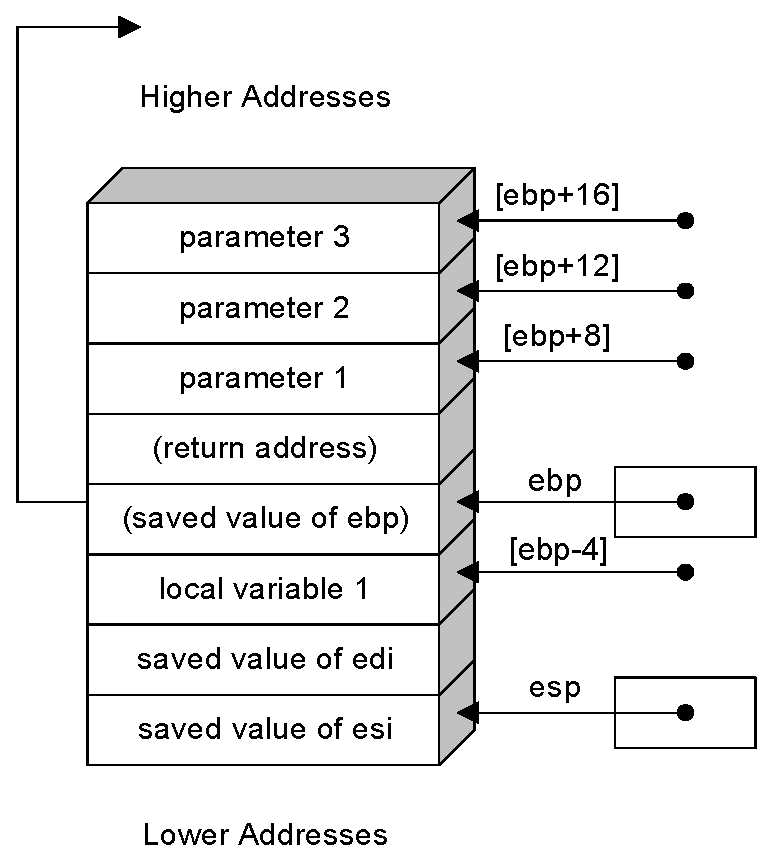
\includegraphics[width=4in]{x86-32bit/x86-activation-record.pdf}
\caption{A picture of the stack in memory during the execution of the body of myFunc}
\label{x86-activation-record.fig}
\end{figure}

The assembly code for {\tt myFunc()} was shown above in
Listing~\ref{x86-callee-example-1.s.lst}. The C++ code to call that
subroutine is shown in
Listing~\ref{x86-callee-example-main.cpp.lst}.

\begin{figure}[h!]
\lstinputlisting[caption={Example C++ code to invoke a 3-parameter x86 subroutine},label={x86-callee-example-main.cpp.lst},backgroundcolor=\color{white},frame=trBL,linewidth=6.9in,xleftmargin=0.15in,language=C++]{x86-32bit/code/callee-example-main.cpp}
\end{figure}







\chapter{64-bit x86 Assembly}

\begin{quotation}
\ldots
\end{quotation}

\noindent {\em This chapter was derived from a document written by Adam Ferrari and later updated by Alan Batson, Mike Lack, Anita
Jones, and Aaron Bloomfield}

\section{Introduction}

This small guide, in combination with the material covered in the
class lectures on assembly language programming, should provide enough
information to do the assembly language labs for this class. In this
guide, we describe the basics of 64-bit x86 assembly language
programming, covering a small but useful subset of the available
instructions and assembler directives. However, real x86 programming
is a large and extremely complex universe, much of which is beyond the
useful scope of this class. For example, there exists real (albeit
older) x86 code running in the world was written using the 16-bit
subset of the x86 instruction set. Using the 16-bit programming model
can be quite complex~-- it has a segmented memory model, more
restrictions on register usage, and so on. This was expanded into a
32-bit programming model in 1985, but that had the limit of only 4 Gb
of memory.  In this guide we'll restrict our attention to the more
modern aspects of 64-bit x86 programming, and delve into the
instruction set only in enough detail to get a basic feel for
programming x86 compatible chips at the hardware level.

\section{Registers}

Modern 64-bit x86 processors have sixteen 64-bit general purpose
registers, as depicted in Figure~\ref{x86-register-diagram.fig}. The
register names for the first eight registers are mostly historical in
nature; the last eight registers were given sequential numbers. For
example, RAX used to be EAX (in the 32-bit machine), which used to be
called the ``accumulator'' since it was used by a number of arithmetic
operations, and RCX (32-bit version: ECX) was known as the ``counter''
since it was used to hold a loop index. Whereas most of the registers
have lost their special purposes in the modern instruction set, by
convention, two are sometimes reserved for special purposes~-- the
stack pointer (RSP) and the base pointer (RBP).

\begin{figure}[h]
\begin{center}
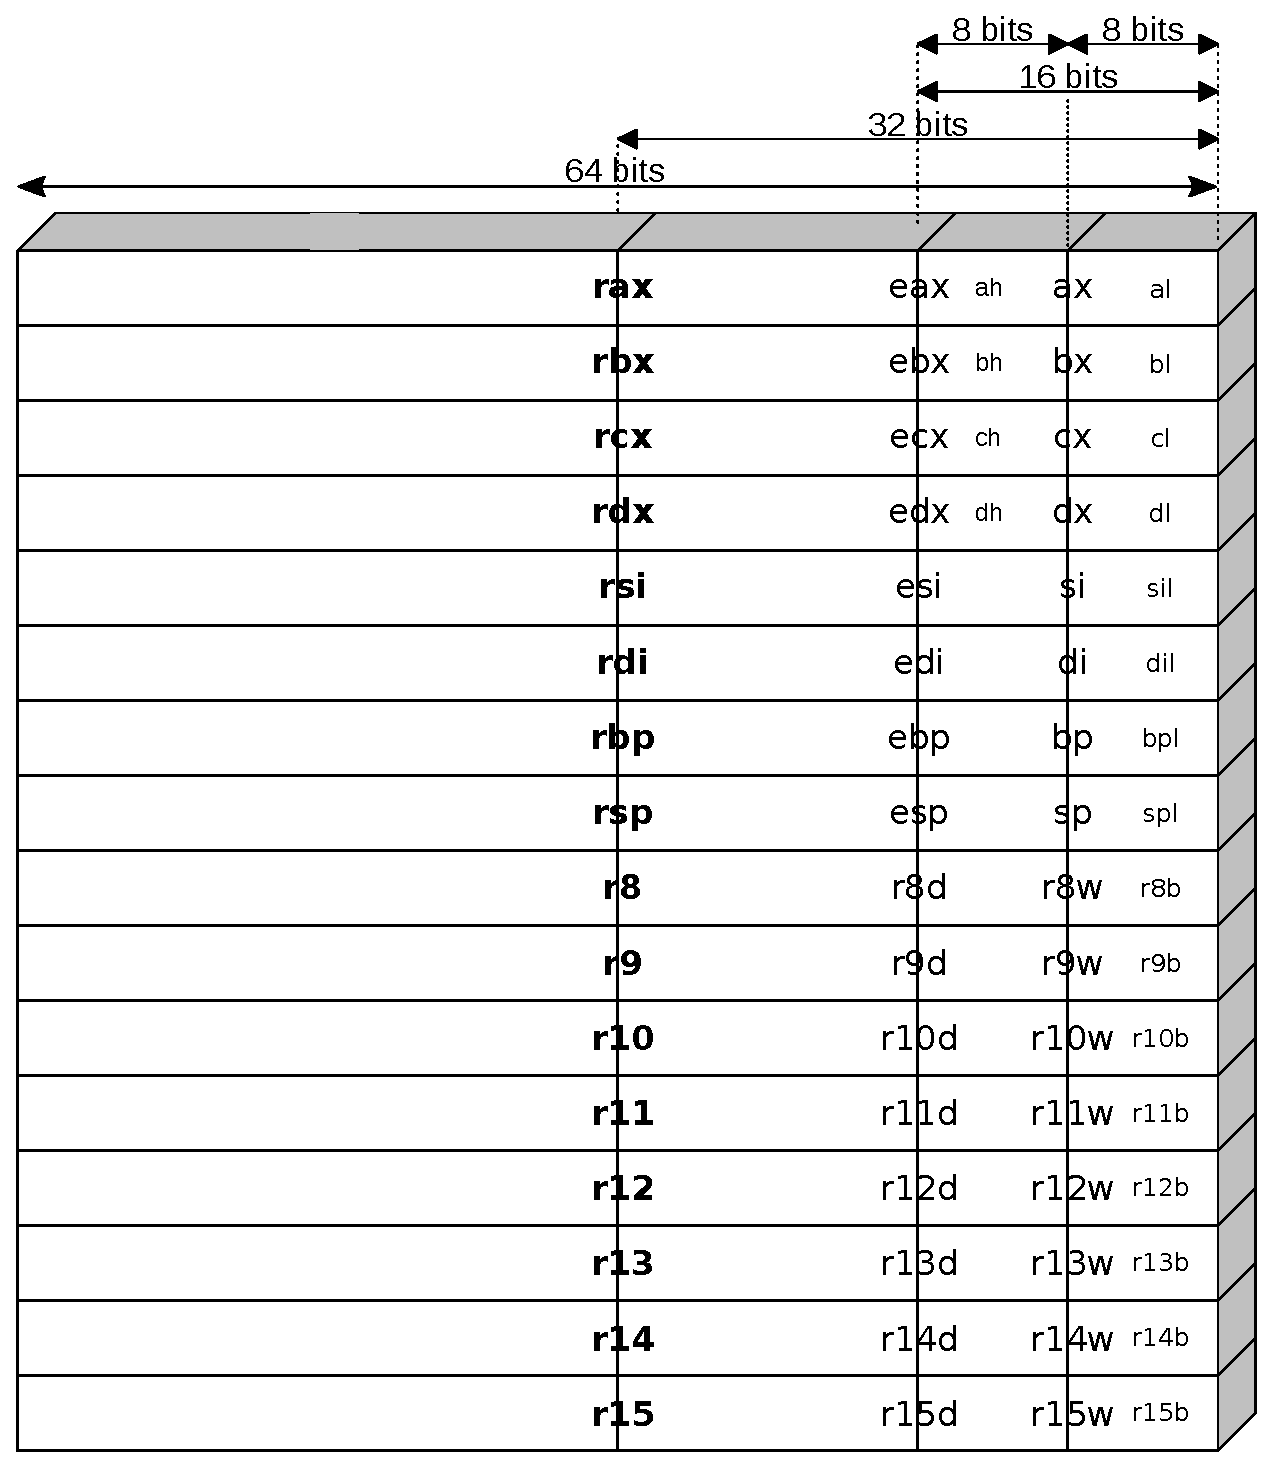
\includegraphics[width=4in]{x86-64bit/x86-register-diagram.pdf}
\end{center}
\caption{The x86 register set}
\label{x86-register-diagram.fig}
\end{figure}

In all cases, subsections of the registers may be used.  For example,
the least significant 2 bytes of RAX can be treated as a 16-bit
register called AX.  The least significant byte of AX can be used as a
single 8-bit register called AL, while the most significant byte of AX
can be used as a single 8-bit register called AH. It is important to
realize that these names refer to the same physical register. When a
two-byte quantity is placed into DX, the update affects the value of
RDX (in particular, the least significant 16 bits of RDX). These
``sub-registers'' are mainly hold-overs from older, 16-bit versions of
the instruction set. However, they are sometimes convenient when
dealing with data that are smaller than 64-bits (e.g., 1-byte ASCII
characters).  Note that four of the registers (EAX, EBX, ECX, and EDX)
have an addition ``sub-register'' spot: the second to last byte of the
register.

When referring to registers in assembly language, the names are not
case-sensitive. For example, the names RAX and rax refer to the same
register.

\section{Memory and Addressing Modes}

\subsection{Declaring Static Data Regions}

You can declare static data regions (analogous to global variables) in
x86 assembly using special assembler directives for this purpose.
Data declarations should be preceded by the .DATA directive. Following
this directive, the directives DB, DW, and DD can be used to declare
one, two, and four byte data locations, respectively. Declared
locations can be labeled with names for later reference - this is
similar to declaring variables by name, but abides by some lower level
rules. For example, locations declared in sequence will be located in
memory next to one another.  Some example declarations are depicted in
Listing~\ref{x86-declaring-memory-regions.lst}.

\begin{figure}[h]
\lstinputlisting[caption=Declaring x86 memory regions,label={x86-declaring-memory-regions.lst},backgroundcolor=\color{white},frame=trBL,linewidth=7in,xleftmargin=0in,language={[x86masm]Assembler}]{x86-64bit/code/memory-regions.s}
\end{figure}

The last example in Listing~\ref{x86-declaring-memory-regions.lst}
illustrates the declaration of an array.  Unlike in high level
languages where arrays can have many dimensions and are accessed by
indices, arrays in assembly language are simply a number of cells
located contiguously in memory. Two other common methods used for
declaring arrays of data are the TIMES directive and the use of string
literals. The TIMES directive tells the assembler to duplicate an
expression a given number of times. For example, the statement ``TIMES
4 DB 2'' is equivalent to ``2, 2, 2, 2''. Some examples of declaring
arrays are depicted in Listing~\ref{x86-declaring-arrays.lst}.

\begin{figure}[h]
\lstinputlisting[caption=Declaring x86 arrays in memory,label={x86-declaring-arrays.lst},backgroundcolor=\color{white},frame=trBL,linewidth=7in,xleftmargin=0in,language={[x86masm]Assembler}]{x86-64bit/code/declaring-arrays.s}
\end{figure}

\subsection{Addressing Memory}
\label{addressing-memory.sec}

Modern x86-compatible processors are capable of addressing up to
$2^{64}$ bytes of memory; that is, memory addresses are 64-bits wide.
For example, in Listings~\ref{x86-declaring-memory-regions.lst} and
\ref{x86-declaring-arrays.lst}, where we used labels to refer to memory
regions, these labels are actually replaced by the assembler with
64-bit quantities that specify addresses in memory. In addition to
supporting referring to memory regions by labels (i.e. constant
values), the x86 provides a flexible scheme for computing and
referring to memory addresses:

{\bf x86 Addressing Mode Rule}~-- Up to two of the 64-bit registers
and a 64-bit signed constant can be added together to compute a memory
address. One of the registers can be optionally pre-multiplied by 2,
4, or 8.

To see this memory addressing rule in action, we'll look at some
example mov instructions.  As we'll see later in
Section~\ref{data-movement-instructions.sec}, the {\tt mov} instruction
moves data between registers and memory.  This instruction has two
operands~-- the first is the destination (where we're moving data {\em
  to}) and the second specifies the source (where we're getting the
data {\em from}). Some examples of mov instructions using address
computations that obey the above rule are shown in
Listing~\ref{x86-valid-addressing-modes.lst}.

\begin{figure}[h]
\lstinputlisting[caption={Valid x86 addressing modes},label={x86-valid-addressing-modes.lst},backgroundcolor=\color{white},frame=trBL,linewidth=7in,xleftmargin=0in,language={[x86masm]Assembler}]{x86-64bit/code/valid-addressing-modes.s}
\end{figure}

Some examples of incorrect address calculations are shown in Listing~\ref{x86-invalid-addressing-modes.lst}.

\begin{figure}[h]
\lstinputlisting[caption={Invalid x86 addressing modes},label={x86-invalid-addressing-modes.lst},backgroundcolor=\color{white},frame=trBL,linewidth=7in,xleftmargin=0in,language={[x86masm]Assembler}]{x86-64bit/code/invalid-addressing-modes.s}
\end{figure}


\subsection{Size Directives}

In general, the intended size of the of the data item at a given
memory address can be inferred from the assembly code instruction in
which it is referenced. For example, in all of the above instructions,
the size of the memory regions could be inferred from the size of the
register operand~-- when we were loading a 64-bit register, the
assembler could infer that the region of memory we were referring to
was 8 bytes wide. When we were storing the value of a one byte
register to memory, the assembler could infer that we wanted the
address to refer to a single byte in memory.  However, in some cases
the size of a referred-to memory region is ambiguous. Consider the
instruction {\tt mov [ebx], 2}.


Should this instruction move the value 2 into the single byte at
address EBX? Perhaps it should move the 64-bit integer representation
of 2 into the 4-bytes starting at address EBX. Since either is a valid
possible interpretation, the assembler must be explicitly directed as
to which is correct.  The size directives {\tt BYTE PTR}, {\tt WORD
  PTR}, {\tt DWORD PTR}, and {\tt QWORD PTR} serve this purpose. For
examples, see Listing~\ref{x86-size-directives.lst}.

\begin{figure}[h]
\lstinputlisting[caption={x86 size directive usage},label={x86-size-directives.lst},backgroundcolor=\color{white},frame=trBL,linewidth=7in,xleftmargin=0in,language={[x86masm]Assembler}]{x86-64bit/code/size-directives.s}
\end{figure}


\section{Instructions}

Machine instructions generally fall into three categories: data movement, arithmetic/logic,
and control-flow. In this section, we will look at important examples of x86 instructions from
each category. This section should not be considered an exhaustive list of x86 instructions, but
rather a useful subset.

In this section, we will use the following notation:

\begin{itemlist}
\item $<$reg64$>$ - means any 64-bit register described in Section 2, for example, ESI.
\item $<$reg16$>$ - means any 16-bit register described in Section 2, for example, BX.
\item $<$reg32$>$ - means any 32-bit register described in Section 2, for example, BX.
\item $<$reg8$>$ - means any 8-bit register described in Section 2, for example AL.
\item $<$reg$>$ - means any of the above.
\item $<$mem$>$ - will refer to a memory address, as described in Section~\ref{addressing-memory.sec}, for example {\tt [EAX]}, or
{\tt [var+4]}, or {\tt DWORD PTR [RAX+RBX]}.
\item $<$con64$>$ - means any 64-bit constant.
\item $<$con32$>$ - means any 32-bit constant.
\item $<$con16$>$ - means any 16-bit constant.
\item $<$con8$>$ - means any 8-bit constant.
\item $<$con$>$ - means any of the above sized constants.
\end{itemlist}

\subsection{Data Movement Instructions}
\label{data-movement-instructions.sec}

\asminstructionsummary{mov}
{mov $<$reg$>$,$<$reg$>$\newline mov $<$reg$>$,$<$mem$>$\newline mov $<$mem$>$,$<$reg$>$\newline mov $<$reg$>$,$<$const$>$\newline mov $<$mem$>$,$<$const$>$}
{The mov instruction moves the data item referred to by its second
  operand (i.e.  register contents, memory contents, or a constant
  value) into the location referred to by its first operand (i.e. a
  register or memory). While register-to-register moves are possible,
  direct memory-to-memory moves are not. In cases where memory
  transfers are desired, the source memory contents must first be
  loaded into a register, then can be stored to the destination memory
  address.}
{mov rax, rbx \linebreak mov BYTE PTR [var], 5 }
{; transfer ebx to eax\linebreak; store the value 5 into the byte at\linebreak; memory location ``var''}
{2.2in}{3.5in}

\asminstructionsummary{push}
{push $<$reg$>$\newline push $<$mem$>$\newline push $<$con64$>$}
{The push instruction places its operand onto the top of the hardware supported
stack in memory. Specifically, push first decrements RSP by 8, then places its
operand into the contents of the 64-bit location at address [RSP]. RSP (the stack
pointer) is decremented by push since the x86 stack grows down~-- i.e. the stack
grows from high addresses to lower addresses.}
{push rax\newline push [var]}
{; push the contents of rax onto the stack\newline
; push the 8 bytes at address ``var'' onto stack}
{1in}{4.7in}

\asminstructionsummary{pop}
{pop $<$reg$>$\newline pop $<$mem$>$}
{The pop instruction removes the 8-byte data element from the top of
  the hardware supported stack into the specified operand (i.e.
  register or memory location). Specifically, pop first moves the 8
  bytes located at memory location [RSP] into the specified register or
  memory location, and then increments SP by 8.}
{pop rdi \newline pop [rbx]}
{; pop the top element of the stack into RDI.\newline
; pop the top element of the stack into memory at\newline
; the four bytes starting at location RBX.}
{1in}{4.7in}

\asminstructionsummary{lea}
{lea $<$reg64$>$,$<$mem$>$}
{The lea instruction places the address specified by its second
  operand into the register specified by its first operand. Note, the
  contents of the memory location are not loaded~-- only the effective
  address is computed and placed into the register.  This is useful
  for obtaining a ``pointer'' into a memory region.}
{lea rax, [var]\newline lea rdi, [rbx+4*rsi]}
{; the address of ``var'' is placed in RAX \newline
; the value RBX+4*RSI is placed in RDI}
{1.85in}{3.85in}

\subsection{Arithmetic and Logic Instructions}

\asminstructionsummary{add, sub}
{add $<$reg$>$,$<$reg$>$ \hspace{0.5in} sub $<$reg$>$,$<$reg$>$ \newline
add $<$reg$>$,$<$mem$>$ \hspace{0.5in} sub $<$reg$>$,$<$mem$>$ \newline
add $<$mem$>$,$<$reg$>$ \hspace{0.5in} sub $<$mem$>$,$<$reg$>$ \newline
add $<$reg$>$,$<$con$>$ \hspace{0.5in} sub $<$reg$>$,$<$con$>$ \newline
add $<$mem$>$,$<$con$>$ \hspace{0.5in} sub $<$mem$>$,$<$con$>$}
{The add instruction adds together its two operands, storing the
  result in its first operand. Similarly, the sub instruction
  subtracts its second operand from its first.  Note, whereas both
  operands may be registers, at most one operand may be a memory
  location.}
{add rax, 10\newline 
sub [var], rsi\newline\newline\newline
add BYTE PTR [var], 10}
{; add 10 to the contents of RAX. \newline
; subtract the contents of RSI from \newline
; the 64-bit integer stored at \newline
; memory location ``var''.\newline
; add 10 to the single byte stored\newline
; at memory address ``var''.\newline}
{2.2in}{3.5in}

\asminstructionsummary{inc, dec}
{inc $<$reg$>$ \hspace{0.5in} dec $<$reg$>$\newline
inc $<$mem$>$ \hspace{0.5in} dec $<$mem$>$}
{The inc instruction increments the contents of its operand by one,
  and similarly dec decrements the contents of its operand by one.}
{dec rax \newline inc DWORD PTR [var]}
{; subtract one from the contents of RAX. \newline
; add one to the 64-bit integer stored at \newline
; memory location ``var''.}
{1.8in}{3.9in}

\asminstructionsummary{imul}
{imul $<$reg64$>$,$<$reg64$>$\newline
imul $<$reg64$>$,$<$mem$>$\newline
imul $<$reg64$>$,$<$reg64$>$,$<$con$>$\newline
imul $<$reg64$>$,$<$mem$>$,$<$con$>$}
{The imul instruction has two basic formats: two-operand (first two
syntax listings above) and three-operand (last two syntax listings
above).  The two-operand form multiplies its two operands together and
stores the result in the first operand. The result (i.e., first)
operand must be a register.  The three operand form multiplies its
second and third operands together and stores the result in its first
operand. Again, the result operand must be a register.  Furthermore,
the third operand is restricted to being a constant value.}
{imul rax, [var]\newline\newline\newline
imul rsi, rdi, 25}
{; multiply the contents of RAX by the \newline
; 64-bit contents of the memory location \newline
; ``var''. Store the result in RAX.\newline
; multiply the contents of RDI by 25. \newline
; Store the result in RSI.}
{1.8in}{3.9in}

\asminstructionsummary{idiv}
{idiv $<$reg64$>$\newline
idiv $<$mem$>$}
{The idiv instruction is used to divide the contents of the 64 bit
  integer RDX:RAX (constructed by viewing RDX as the most significant
  eight bytes and RAX as the least significant eight bytes) by the
  specified operand value. The quotient result of the division is
  stored into RAX, while the remainder is placed in RDX. This
  instruction must be used with care. Before executing the
  instruction, the appropriate value to be divided must be placed into
  RDX and RAX. Clearly, this value is overwritten when the idiv
  instruction is executed.}
{idiv rbx \newline\newline\newline idiv DWORD PTR [var]}
{; divide the contents of RDX:RAX by the \newline
; contents of RBX. Place the quotient \newline
; in RAX and the remainder in RDX.\newline
; same as above, but divide by the \newline
; 64-bit value stored at memory \newline
; location ``var''.}
{1.9in}{3.8in}

\asminstructionsummary{and, or, xor}
{and $<$reg$>$,$<$reg$>$ \hspace{0.25in} or $<$reg$>$,$<$reg$>$ \hspace{0.25in} xor $<$reg$>$,$<$reg$>$ \newline
and $<$reg$>$,$<$mem$>$ \hspace{0.25in} or $<$reg$>$,$<$mem$>$ \hspace{0.25in} xor $<$reg$>$,$<$mem$>$ \newline
and $<$mem$>$,$<$reg$>$ \hspace{0.25in} or $<$mem$>$,$<$reg$>$ \hspace{0.25in} xor $<$mem$>$,$<$reg$>$ \newline
and $<$reg$>$,$<$con$>$ \hspace{0.25in} or $<$reg$>$,$<$con$>$ \hspace{0.25in} xor $<$reg$>$,$<$con$>$ \newline
and $<$mem$>$,$<$con$>$ \hspace{0.25in} or $<$mem$>$,$<$con$>$ \hspace{0.25in} xor $<$mem$>$,$<$con$>$}
{These instructions perform the specified logical operation (logical
bitwise and, or, and exclusive or, respectively) on their operands,
placing the result in the first operand location.}
{and rax, 0fH \newline xor rdx, rdx}
{; clear all but the last 4 bits of RAX. \newline ; set the contents of RDX to zero.}
{1.7in}{4in}

\asminstructionsummary{not}
{not $<$reg$>$ \newline not $<$mem$>$}
{Performs the logical negation of the operand contents (i.e., flips all bit values).}
{not BYTE PTR [var]}
{; negate all bits in the byte at the \newline ; memory location ``var''.}
{1.7in}{4in}

\asminstructionsummary{neg}
{neg $<$reg$>$ \newline neg $<$mem$>$}
{Performs the arithmetic (i.e., two's complement) negation of the operand contents.}
{neg rax \newline neg [var]}
{; negate the contents of RAX. \newline ; negate the contests of ``var''}
{1.4in}{4.3in}

\asminstructionsummary{shl, shr}
{shl $<$reg$>$,$<$con8$>$ \hspace{0.5in} shr $<$reg$>$,$<$con8$>$\newline
shl $<$mem$>$,$<$con8$>$ \hspace{0.5in} shr $<$mem$>$,$<$con8$>$\newline
shl $<$reg$>$,cl \hspace{0.92in} shr $<$reg$>$,cl\newline
shl $<$mem$>$,cl \hspace{0.92in} shr $<$mem$>$,cl}
{These instructions shift the bits in their first operand's contents
  left and right ({\tt shl} and {\tt shr}, respectively), padding the
  resulting empty bit positions with zeros. The shifted operand can be
  shifted up to 31 places. The number of bits to shift is specified
  by the second operand, which can be either an 8-bit constant or the
  register CL. In either case, shifts counts of greater then 31 are
  performed modulo 64.}
{shl rax 5 \newline\newline shr [var] 3}{; shift the contents of rax left by 5 bit \newline ; positions \newline ; shift the contents of ``var'' right by 3 \newline ; bit positions}{1.4in}{4.3in}

\subsection{Control Flow Instructions}

In this section, we will refer to labeled locations in the program
text as $<$label$>$. Labels can be inserted anywhere in x86 assembly
code text by entering a label name followed by a colon. For example,
consider the code fragment in Listing~\ref{x86-labeled-code-location.lst}.
The second instruction in this code fragment is labeled ``begin''.
Elsewhere in the code, we can refer to the memory location that this
instruction is located at in memory using the more convenient symbolic
name ``begin'' instead of having to refer to the memory address as an
integer.

\begin{figure}[h]
\lstinputlisting[caption={x86 labeled code location},label={x86-labeled-code-location.lst},backgroundcolor=\color{white},frame=trBL,linewidth=4.75in,xleftmargin=2.25in,language={[x86masm]Assembler}]{x86-64bit/code/labeled-code-location.s}
\end{figure}


\asminstructionsummary{jmp}
{jmp $<$label$>$}
{Transfers program control flow to the instruction at the memory
  location indicated by the operand.}
{jmp begin}{; jumps to the ``begin'' label}
{1.5in}{3.7in}

\asminstructionsummary{jCC}
{je $<$label$>$ ; Jump when equal\newline
jne $<$label$>$ ; Jump when not equal\newline
jz $<$label$>$ ; Jump when last result was zero\newline
jg $<$label$>$ ; Jump when greater than\newline
jge $<$label$>$ ; Jump when greater than or equal to\newline
jl $<$label$>$ ; Jump when less than\newline
jle $<$label$>$ ; Jump when less than or equal to}
{These instructions are conditional jumps that are based on the status
  of a set of {\bf condition codes} that are stored in a special
  register called the {\em machine status word}. The contents of the
  machine status word include information about the last arithmetic
  operation performed. For example, one bit of this word indicates if
  the last result was zero. Another indicates if the last result was
  negative.  Based on these condition codes, a number of conditional
  jumps can be performed. For example, the jz instruction performs a
  jump to the specified operand label if the result of the last
  arithmetic operation (e.g. add, sub, etc.) was zero. Otherwise,
  control proceeds to the next instruction in sequence after the jz.
  These conditional jumps are the underlying support needed to
  implement high-level language features such as ``if'' statements and
  loops (e.g. ``while'' and ``for''). \vspace{6pt}\newline
  A number of the conditional branches are given names that are
  intuitively based on the last operation performed being a special
  compare instruction, cmp (see below).  For example, conditional
  branches such as jle and jne are based on first performing a cmp
  operation on the desired operands.}
{cmp rax, rbx \newline jle done}
{; if the contents of rax are less than or \newline
; equal to the contents of ebx, jump to the \newline
; code location labeled ``done''.}
{1.4in}{4.3in}

\asminstructionsummary{cmp}
{cmp $<$reg$>$,$<$reg$>$\newline
cmp $<$reg$>$,$<$mem$>$\newline
cmp $<$mem$>$,$<$reg$>$\newline
cmp $<$reg$>$,$<$con$>$\newline
cmp $<$mem$>$,$<$con$>$}
{Compares the two specified operands, setting the condition codes in
  the machine status word appropriately. In fact, this instruction is
  equivalent to the sub instruction, except the result of the
  subtraction is discarded.}
{cmp DWORD PTR [var], 10\newline jeq loop}
{; if the 4 bytes stored at memory\newline
; location ``var'' equal the 4-byte\newline
;  integer value 10, then jump to the\newline
; code location labeled loop}
{2.2in}{3.5in}

\asminstructionsummary{call}
{call $<$label$>$}
{This instruction implements a subroutine call that operates in
cooperation with the subroutine return instruction, ret, described
below. This instruction first pushes the current code location onto
the hardware supported stack in memory (see the push instruction for
details), and then performs an unconditional jump to the code location
indicated by the label operand. The added value of this instruction
(as compared to the simple jmp instruction) is that it saves the
location to return to when the subroutine completes.}
{call my\_subroutine}
{; jumps to the ``my\_subroutine'' label, \newline
; pushing the return address onto the \newline
; stack}
{1.8in}{3.9in}

\asminstructionsummary{ret}
{ret}
{In cooperation with the call instruction, the ret instruction
  implements a subroutine return mechanism. This instruction first
  pops a code location off the hardware supported in-memory stack (see
  the pop instruction for details). It then performs an unconditional
  jump to the retrieved code location.}
{ret}{; returns to the address on the top of the stack}
{1in}{4.7in}


\section{Basic Program Structure}
\label{x86-basic-program-structure.sec}

\begin{wrapfigure}{r}{0.37\textwidth}
\lstinputlisting[backgroundcolor=\color{white},frame=trBL,linewidth=2.5in,xleftmargin=0.25in,label={x86-return2.s.lst},language={[x86masm]Assembler},caption={x86 code to return 2}]{x86-64bit/code/return2.s}
\vspace{-0.25in}
\end{wrapfigure}

Given the above repertoire of instructions, you are in a position to
examine the basic skeletal structure of an assembly language
subroutine suitable for linking into C++ code. Unlike C++, which is
often used for the development of complete software systems, assembly
language is most often used in cooperation with other languages such
as Fortran, C, and C++. Commonly, most of a project is implemented in
the more convenient high-level language, and assembly language is used
sparingly to implement extremely low-level hardware interfaces or
performance-critical ``inner loops.'' Thus, in addition to
understanding how to program in assembly language, it is equally
important to understand how to link assembly language code into
high-level language programs.

Before examining the linkage conventions, we must first examine the
basic structure of an assembly language file. To do this, we can
compare a very simple assembly language file to an equivalent C++
file. In Listings~\ref{x86-return2.s.lst} and \ref{x86-return2.cpp.lst} we see
two files, one in C++, the other in x86 assembly. Each file includes a
function (albeit an ugly one) to return the integer value 2.

Note that the fucntion shown in assembly in
Listing~\ref{x86-return2.s.lst} returns a 32-bit value, since it is
put into register eax.  This corresponds to retnring an {\tt int} in C
or C++.  If we wanted to return a 64-bit value, which corresponds to
returning a {\tt long}, then we would put the return value into rax.

The top of the assembly file contains two directives that indicate the
instruction set and memory model we will use for all work in this
class (note, there are other possibilities~-- one might use only the
older 80286 instruction set for wider compatibility, for example).

Next, where in the C++ file we find the declaration of the global
variable ``var'', in the assembly file we find the use of the .DATA
and DD directives (described in Section 3.1) to reserve and initialize
a 4-byte (i.e., integer-sized) memory region labeled ``var''.

\begin{wrapfigure}{r}{0.37\textwidth}
\lstinputlisting[backgroundcolor=\color{white},frame=trBL,linewidth=2.5in,xleftmargin=0.25in,label={x86-return2.cpp.lst},language=C++,caption={C++ code to return 2}]{x86-64bit/code/return2.cpp}
\vspace{-0.25in}\end{wrapfigure}

Next in each file, we find the declaration of the function named
returnTwo. In the C++ file we have declared the function to be extern
``C''. This declaration indicates that the C++ compiler should use C
naming conventions when labeling the function returnTwo in the
resulting object file that it produces. In fact, this naming
convention means that the function returnTwo should map to the label
\_returnTwo in the object code. In the assembly code, we have labeled
the beginning of the subroutine \_returnTwo using the PROC directive,
and have declared the label \_returnTwo to be public. Again, the
result of these actions will be that the subroutine will map to the
symbol \_returnTwo in the object code that the assembler generates.

The function bodies are straight-forward. As we will see in more
detail in Section 6, return values for functions are placed into EAX
by convention, hence the instruction to move the contents of ``var''
into EAX in the assembly code.

\begin{wrapfigure}{r}{0.48\textwidth}
\lstinputlisting[backgroundcolor=\color{white},frame=trBL,linewidth=4in,xleftmargin=0.25in,label={x86-calling-return2.cpp.lst},language=C++,caption={Calling returnTwo() from C++}]{x86-64bit/code/calling-return2.cpp}
\vspace{-0.25in}
\end{wrapfigure}

Given these equivalent function definitions, use of either version of
the function is the same.  A sample call to the function returnTwo is
depicted in Listing~\ref{x86-calling-return2.cpp.lst}. This C++ code
could be linked to either definition of the function and would produce
the same results (note, we could not link to both definitions, or the
linker would produce a ``multiply defined symbol'' error. The
mechanics of program linking will be discussed in an associated
document that relates to the specific programming environment that you
will use to assemble and run programs.


\chapter{The 64-bit x86 C Calling Convention}

\begin{quotation}
\ldots
\end{quotation}

\noindent {\em This chapter was derived from a document written by Adam Ferrari and later updated by Alan Batson, Mike Lack, Anita
Jones, and Aaron Bloomfield}

\section{What is a Calling Convention?}

At the end of the previous chapter, we saw a simple example of a
subroutine defined in x86 assembly language. In fact, this subroutine
was quite simple~-- it did not modify any registers except EAX (or
RAX) (which was needed to return the result), and it did not call any
other subroutines. In practice, such simple function definitions are
rarely useful. When more complex subroutines are combined in a single
program, a number of complicating issues arise.  For example, how are
parameters passed to a subroutine? Can subroutines overwrite the
values in a register, or does the caller expect the register contents
to be preserved? Where should local variables in a subroutine be
stored? How should results be returned from functions?

To allow separate programmers to share code and develop libraries for
use by many programs, and to simplify the use of subroutines in
general, programmers typically adopt a common {\em calling
  convention}. The calling convention is simply a set of rules that
answers the above questions without ambiguity to simplify the
definition and use of subroutines. For example, given a set of calling
convention rules, a programmer need not examine the definition of a
subroutine to determine how parameters should be passed to that
subroutine. Furthermore, given a set of calling convention rules,
high-level language compilers can be made to follow the rules, thus
allowing hand-coded assembly language routines and high-level language
routines to call one another.

In practice, even for a single processor instruction set, many calling
conventions are possible.  In this class we will examine and use one
of the most important conventions: the C language calling convention.
Understanding this convention will allow you to write assembly
language subroutines that are safely callable from C and C++ code, and
will also enable you to call C library functions from your assembly
language code.

\section{The C Calling Convention}

The C calling convention is based heavily on the use of the
hardware-supported stack. To understand the C calling convention, you
should first make sure that you fully understand the push, pop, call,
and ret instructions~-- these will be the basis for most of the rules.
In this calling convention, subroutine parameters are passed on the
stack. Registers are saved on the stack, and local variables used by
subroutines are placed in memory on the stack. In fact, this
stack-centric implementation of subroutines is not unique to the C
language or the x86 architecture. The vast majority of high-level
procedural languages implemented on most processors have used similar
calling convention.

The calling convention is broken into two sets of rules. The first set
of rules is employed by the caller of the subroutine, and the second
set of rules is observed by the writer of the subroutine (the
``callee''). It should be emphasized that mistakes in the observance
of these rules quickly result in fatal program errors; thus meticulous
care should be used when implementing the call convention in your own
subroutines.

\section{The Caller's Rules}

The caller should adhere to the following rules when invoking a
subroutine:

\begin{numlist}
\item Before calling a subroutine, the caller should save the contents
  of certain registers that are designated caller-saved. The
  caller-saved registers are r10, r11, and any registers that
  parameters are put into. If you want the contents of these registers
  to be preserved across the subroutine call, push them onto the
  stack.
\item To pass parameters to the subroutine, we put up to six of them
  into registers (in order: rdi, rsi, rdx, rcx, r8, r9).  If there are
  more than six parameters to the subroutine, then push the rest onto
  the stack in {\em reverse order} (i.e. last parameter first)~--
  since the stack grows down, the first of the extra parameters
  (really the seventh parameter) parameter will be stored at the
  lowest address (this inversion of parameters was historically used
  to allow functions to be passed a variable number of parameters).
\item To call the subroutine, use the {\tt call} instruction. This
  instruction places the return address on top of the parameters on
  the stack, and branches to the subroutine code.
\item After the subroutine returns, (i.e. immediately following the
  call instruction) the caller must remove any additional parameters
  (beyond the six stored in registers) from stack.  This restores the
  stack to its state before the call was performed.
\item The caller can expect to find the return value of the subroutine
  in the register RAX.
\item The caller restores the contents of caller-saved registers (r10,
  r11, and any in the parameter passing registers) by popping them off
  of the stack. The caller can assume that no other registers were
  modified by the subroutine.
\end{numlist}

Due to the way the calling convention is structured, it will typically
be the case that some (or most) of these steps will not make any
changes to the stack.  For example, if there are six or fewer
parameters, then nothing is pushed onto the stack in that step.
Likewise, programmers (and compilers) tyipcally keep the results they
care about out of the caller-saved registers in steps 1 and 6 to
prevent excess pushes and pops.

\section{The Callee's Rules}

The definition of the subroutine should adhere to the following rules:

\begin{numlist}

\item Allocate local variables by using registers or making space on
  the stack.  Recall, the stack grows down, so to make space on the
  top of the stack, the stack pointer should be decremented. The
  amount by which the stack pointer is decremented depends on the
  number of local variables needed. For example, if a local {\tt
    float} and a local {\tt long} (12 bytes total) were required, the
  stack pointer would need to be decremented by 12 to make space for
  these local variables:

\begin{lstlisting}[backgroundcolor=\color{white},frame=trBL,linewidth=3.75in,xleftmargin=2.25in,label={x86-callee-code-2.lst},language={[x86masm]Assembler},caption={x86 callee code, part 2}]
sub rsp, 12
\end{lstlisting}

As with parameters, local variables will be located at known offsets
from the stack pointer.

\item Next, the values of any registers that are designated
  callee-saved that will be used by the function must be saved. To
  save registers, push them onto the stack. The callee-saved registers
  are RBX, RBP, and R12 through R15 (RSP will also be preserved by the
  call convention, but need not be pushed on the stack during this
  step).

  After these three actions are performed, the actual operation of the
  subroutine may proceed.  When the subroutine is ready to return, the
  call convention rules continue:

\item When the function is done, the return value for the function
  should be placed in RAX if it is not already there.

\item The function must restore the old values of any callee-saved
  registers (RBX, RBP, and R12 through R15) that were modified. The
  register contents are restored by popping them from the stack. Note,
  the registers should be popped in the inverse order that they were
  pushed.

\item Next, we deallocate local variables. The easiest way to do this
  is to add to RSP the same amount that was subtracted from it in step
  1.

\item Finally, we return to the caller by executing a {\tt ret}
  instruction. This instruction will find and remove the appropriate
  return address from the stack.

\end{numlist}

If you look at the assembly generated by some compilers, you will see
a few extra commands in there in the callee's prologue:

\begin{lstlisting}[backgroundcolor=\color{white},frame=trBL,linewidth=5.5in,xleftmargin=1.25in,label={x86-callee-code-2.lst},language={[x86masm]Assembler},caption={x86 extraneous codedd}]
push rbp       ; at the start of the callee
mov rbp, rsp
...
pop rbp        ; just before the ending 'ret'
\end{lstlisting}

This code is unnecessary, and is a hold-over from the 32-bit calling
convention.  You can tell the compiler to not include this code by
invoking it with the {\tt -fomit-frame-pointer} flag.

It might be noted that the callee's rules fall cleanly into two halves
that are basically mirror images of one another. The first half of the
rules apply to the beginning of the function, and are therefor
commonly said to define the {\em prologue} to the function. The latter
half of the rules apply to the end of the function, and are thus
commonly said to define the {\em epilogue} of the function.

\section{Calling Convention Example}

The above rules may seem somewhat abstract on first examination. In practice, the rules
become simple to use when they are well understood and familiar. To start the process of better
understanding the call convention, we now examine a simple example of a subroutine call and a
subroutine definition.

\begin{figure}[h!]
\lstinputlisting[caption={Example function call, caller's rules obeyed},label={x86-caller-example-1.s.lst},backgroundcolor=\color{white},frame=trBL,linewidth=6in,xleftmargin=0.75in,language={[x86masm]Assembler}]{x86-64bit/code/caller-example-1.s}
\end{figure}


In Listing~\ref{x86-caller-example-1.s.lst} a sample function call is
depicted. The three parameters are put into the parameter passing
registers; if there were more than 6, then the additional ones would
be pushed onto the stack in reverse order.  The call instruction is
used to jump to the beginning of the subroutine in anticipation of the
fact that the subroutine will use the ret instruction to return when
the subroutine completes. When the subroutine returns, the parameters
must be removed from the stack. A simple way to do this is to add the
appropriate amount to the stack pointer (since the stack grows down).
Finally, the result is available in RAX.

Next up is the caller's rules. An example subroutine implementation
that obeys the callee's rules is depicted in
Listing~\ref{x86-callee-example-1.s.lst}. The subroutine prologue
performs the standard actions of allocating local variables by
decrementing the stack pointer, and saving register values on the
stack.

\begin{figure}[h!]
\lstinputlisting[caption={Example function definition, callee's rules obeyed},label={x86-callee-example-1.s.lst},backgroundcolor=\color{white},frame=trBL,linewidth=6.9in,xleftmargin=0.15in,language={[x86masm]Assembler}]{x86-64bit/code/callee-example-1.s}
\end{figure}

In the body of the subroutine we can see how the local variables are
accessed.  The prologue put 24 bytes of ``stuff'' onto the stack:
three 8 byte values.  The first was the local variable (via the {\tt
  sub rsp, 8} call).  The second was the rbx backup, and the third was
the rbp backup.  Thus, the stack pointer is now 16 bytes below the
local variable, as two 8 byte ``things'' have been pushed onto the
stack since the local variable was allocated.  Thus, to access the
local variable, one uses {\tt [rsp+16]}, as seen throughout the code.

The function epilogue, as expected, is basically a mirror image of the
function prologue. The caller's register values are recovered from the
stack, the local variables are deallocated by resetting the stack
pointer, and the {\tt ret} instruction is used to return to the
appropriate code location in the caller.

A good way to visualize the operation of the calling convention is to
draw the contents of the nearby region of the stack during subroutine
execution. Figure~\ref{x86-activation-record.fig} depicts the contents
of the stack during the execution of the body of myFunc (myFunc is
depicted in Listing~\ref{x86-callee-example-1.s.lst}). Notice, lower
addresses are depicted lower in the figure, and thus the ``top'' of
the stack is the bottom-most cell. This corresponds visually to the
intuitive statement that the x86 hardware stack ``grows down.'' The
cells depicted in the stack are 64-bit wide memory locations, thus the
memory addresses of the cells are 4 bytes apart. From this picture we
see clearly why the first parameter resides at an offset of 8 bytes
from the base pointer. Above the parameters on the stack (and below
the base pointer), the call instruction placed the return address,
thus leading to an extra 4 bytes of offset from the base pointer to
the first parameter.

\begin{figure}[h]
\centering
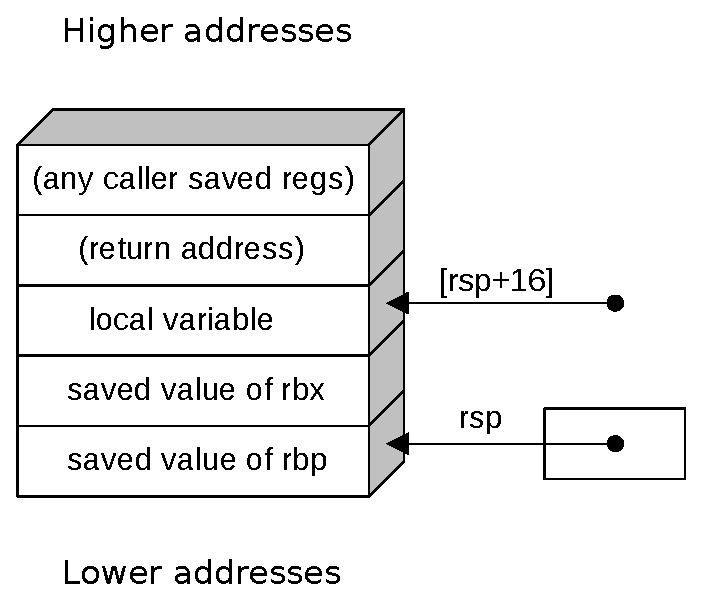
\includegraphics[width=4in]{x86-64bit/x86-activation-record.pdf}
\caption{A picture of the stack in memory during the execution of the body of myFunc}
\label{x86-activation-record.fig}
\end{figure}

The assembly code for {\tt myFunc()} was shown above in
Listing~\ref{x86-callee-example-1.s.lst}. The C++ code to call that
subroutine is shown in
Listing~\ref{x86-callee-example-main.cpp.lst}.

\begin{figure}[h!]
\lstinputlisting[caption={Example C++ code to invoke a 3-parameter x86 subroutine},label={x86-callee-example-main.cpp.lst},backgroundcolor=\color{white},frame=trBL,linewidth=6.9in,xleftmargin=0.15in,language=C++]{x86-64bit/code/callee-example-main.cpp}
\end{figure}







\part{Applications}

\chapter{Huffman Coding}

\lstset{frameround=fttt,captionpos=b}

% Chapter by Charles Eckman, cceckman@gmail.com

% Below macro for above/below from Andrey Vihrov 
% http://tex.stackexchange.com/questions/32285/referencing-to-above-or-below
\makeatletter
\newcount\here@undef
\newcommand{\here}[1]{%
  \@ifundefined{here@#1@undef}{}{\advance\here@undef by -1}%
  \@namedef{here@#1}{}}
\newcommand{\where}[1]{%
  \@ifundefined{here@#1}{%
    below%
    \@ifundefined{here@#1@undef}{%
      \@namedef{here@#1@undef}{}%
      \advance\here@undef by 1
    }{}%
  }{%
    above%
  }%
}
\AtEndDocument{%
  \ifnum\here@undef>0
    \GenericWarning{}{There were undefined above/below labels}%
  \fi}
\makeatother

\section{Introduction: the compression problem}

% IMAGE - Screenshot from Doctor Who

Let's start off this chapter with some math. (Don't worry, we'll get back to programming soon.)

The image \where{dw-screencap} is one frame of a video (specifically, an episode of the British television programme \textit{Doctor Who}). You're interested in downloading this video, but your hard drive is filling up. How much space would you expect the video to take up?

We can estimate by figuring out the information content of the video. Every
frame is 1920 by 1080 pixels; each pixel is at least three bytes (eight bits of
red, eight bits of blue, and eight bits of green.) For video to appear smooth to
the human eye, it must have a minimum framerate of about 30 frames per second (fps); however, some television is shot at 24 fps. The video is 2882 seconds long.

%$$
%& \frac{8 \text{ bits}}{1 \text{ byte}} \times 
%\frac{3 \text{ bytes}}{1 \text{ pixel}} \times
%\frac{1920 \times 1080 \text{ pixels}}{1 \text{frame} \times
%\frac{24 \text{ frames}}{1 \text{ second}} \times
%2882 \text{ seconds} \\
%= & 3442242355200 \text{ bits} \\
%\approx & 400 \text{ gigabytes}
%$$

By this calculation, a 50-minute, high-definition, television episode should amount to 400 gigabytes of data. And yet, the actual file is only about 1.5 gigabytes. Where did all the information go?

Well- nowhere. The above calculation is only relevant if every single bit would change the resulting message, \textit{and} if there are no patterns that can be expressed in a shorter way. Though one may not realize it just by watching, video does have patterns. Adjacent pixels (in space and time) tend towards groups of similarity, with lines (edges) of contrast and motion. Some very clever people have come up with ways to reduce the overall size, without actually losing information; the computer just has to do some work to do.

Compression is a form of \textit{encoding}: a mapping from one representation of information to another representation. Different representations may take up more or less space, but may take less or more time to interpret. Take, for example, the Latin alphabet. Humans are very good at recognizing Latin characters and words when depicted in graphical form. Computers, however, may have trouble recognizing these. On the other hand, a computer can easily deal with the ASCII encoding of a string, while most humans would have difficulty reading a book bit-by-bit. Note also that a two-dimensional graphic takes up more space than a one-dimensional ASCII encoding; this is why a scanned page of, say, a book takes up more space than an original digital document.

% FIGURE: A CAPTCHA
% FIGURE: ASCII ENCODING OF A CAPTCHA

% FIGURE: Scan of a printout of this page.
% FIGURE: Screen capture of this .TEX file.

Compression embodies a longstanding tradeoff in computing between space and time. For many problems, the computer can store a small set of inputs to a function, and re-compute the large set of outputs as needed. Alternatively, it can save the re-computation time by storing the outputs and referring to them as needed. Compression and decompression take time and energy, but they allow data to take up less space when not in use.

\section{Text compression}

Music, video, and image media have numerous attributes related to representation and perception that encourage specialized compression algorithms- so let's make it easy and look at plain text.

\begin{quotation}
Let's imagine a language which has only two valid sentences, and every tweet must be one of the two sentences. They are:

\begin{enumerate}
\item {\em“There’s a horse in aisle five.”}
\item {\em“My house is full of traps.”}
\end{enumerate}

Twitter would look like this:

\begin{figure}[h]
\begin{center}
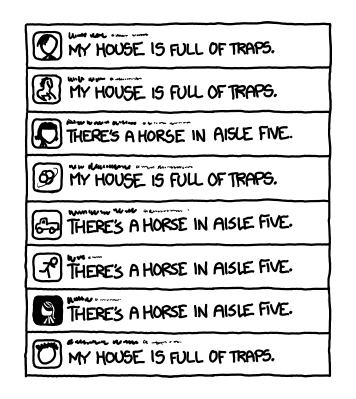
\includegraphics[width=4in]{huffman/twitter-screenshot.png}
\end{center}
\caption{caption} %xkcd what-if \# 34: http://what-if.xkcd.com/34/ (released under a CC BY-NC license)}
\end{figure}

%\image{xkcd-what-if-34-twitter_screenshot.png}

The messages are relatively long, but there’s not a lot of information in each one - all they tell you is whether the person decided to send the trap message or the horse message. It's a 1 or a 0. Although there are a lot of letters, for a reader who knows the pattern the language carries only one bit of information per sentence.

This example hints at a very deep idea, which is that information is fundamentally tied to the recipient’s uncertainty about the message’s content and their ability to predict it in advance.

Claude Shannon - who almost singlehandedly invented modern information theory — had a clever method for measuring the information content of a language. He showed groups of people samples of typical written English which were cut off at a random point, then asked them to guess which letter came next.

Based on the rates of correct guesses - and rigorous mathematical analysis - Shannon determined that the information content of typical written English was around 1.0 to 1.2 bits per letter. This means that a good compression algorithm should be able to compress ASCII English text - which is eight bits per letter - to about 1/8th of its original size. Indeed, if you use a good file compressor on a .txt ebook, that’s about what you'll find.

-- Randall Munroe, in 'what if?'\cite{xkcd-what-if-34}
\end{quotation}

Let's dive into this a little more. If all parties involved know that 0 means "There's a horse in aisle five." and that 1 means "My house is full of traps.", those parties can communicate those two messages very efficiently.\footnote{Furthermore, the 1990 film \textit{Home Alone} could be compressed into Macaulay Culkin repeating "1".} There is some setup involved in ensuring all parties understand this coding; furthermore, the language of expression is limited to those two phrases, which are not very useful in most circumstances.

How do we expand the language of discourse- say, to all of English? Instead of mapping two numbers (0 and 1) to two phrases, let's try mapping numbers to words. We can use an old cryptographic technique called a \textit{dictionary cypher}: everyone involved in the communication has the same edition of the same book. A word is written as a page number, followed by a word number on that page: "43 24" refers to the 24th word on page 43.

This dictionary cypher is an encoding; however, is it necessarily a compression? To determine this, we have to look at the information transmitted versus the information content of the uncompressed message. We must include the transmission of the dictionary (to ensure that both the sender and recevier has a copy), as well as the individual message.

An efficient book to use would be the \textit{Scrabble Players Dictionary}, which includes "More than 100,000\ldots words" on 720 pages. Since this book does not contain definitions few, if any, words are repeated. 
% http://www.merriam-webster.com/cgi-bin/book.pl?scrabdic.htm&3
720 pages can be indexed by 10 bits ($2^{10}=1024$), and each page can be indexed by an 8-bit number ($\frac{100000}{720}=139$, $2^7 < 139 < 2^8$). Thus, any word can be compressed into 18 bits using this dictionary cypher.

This is an improvement over ASCII's 7-bit-per-character coding only for words over three characters. Furthermore, there's a very high overhead in transmitting the entire dictionary; though there are few repeated words, many (really, most) of the words in the dictionary won't be used. 

\section{The prefix tree}

What we'd like to create is an algorithm for coding and decoding that will respond to the particular message transmitted. We can do this by creating a per-message dictionary: we'll transmit only those entries which the current message uses.

The Huffman algorithm generates this dictionary using a data structure called a \textit{prefix tree}. A prefix tree is a binary tree with this additional property:
\begin{quotation}
\textbf{Prefix tree property:} Every node has either two children or none.
\end{quotation}
Phrased slightly differently, {\em every non-leaf node has two children}.

\begin{figure}[prefix-tree]
\end{figure}
\begin{figure}[not-a-prefix-tree]
\end{figure}
% TODO diagrams
Thus, the diagram on the {left right} is a prefix tree; the diagram on the {right left} is not, because node X has only one child.

Why is this property useful? Let's look at what we'll call the \textit{path string} of a node. In a binary tree, this is the sequence of left-and-right traversals (expessed as a sequence of 0s and 1s) that lead from the root of the tree to a given node. For instance, in figure \ref{prefix-tree}, the path string of R is "001", and the path string of M is "01".

The path string of one node is always a \textit{prefix} of its children's path strings, and their children's, etc. By prefix, we mean that each child's string is constructed by appending a 0 or 1 to the parent's path string.

In a prefix tree, every path string is either the prefix to a leaf's path string, or is a leaf's path string. We say that these leaf nodes have \textit{prefix strings}, because they (somewhat confusingly) are \textit{not} the prefix to any other path string.

\begin{quotation}
\textbf{Prefix string property:} If the prefix tree property holds, no path string of a leaf is a prefix to any other path string.
\end{quotation}

A formal proof is beyond the scope of this chapter, but you should convince yourself it's correct.

So given a prefix tree whose leaves correspond to symbols, we can unambiguously translate a binary string of any length into a series of symbols. Our program reads one bit at a time from the input string and moves an indicator left or right down the tree as directed. When it reaches a leaf node, it outputs that symbol and resets the indicator to the head of the tree.

The above paragraph is all that Huffman decoding requires. Let's run through an example.

% TODO example

\section{Huffman encoding}

Huffman encoding is a slightly more elaborate process. We need to construct not just any old prefix tree, but one that will result in an encoded message shorter than the original.

We begin by selecting our set of symbols. In this example, we'll use ASCII characters; it's possible that for some messages, words or phrases could be result in a shorter compressed message.

% TODO complete

\section{Additional reading}

In the introduction of this chapter, we discussed a compression that reduced the size without loss of information. In fact, many media encodings are \textit{lossy}: they do not perfectly preserve the input data. The MP3 music codec, H.264 video codec, and JPEG image format are all (at least optionally) lossy encodings. They exploit the fact that humans have limited perceptive abilities to remove differences that the consumer (audience) might not be able to percieve, in addition to using other compression techniques.

The Huffman encoding we explore in this chapter relies on having access to the entire unencoded message before producing the encoded message. Not all encodings have this property: stream algorithms attempt to encode data in a single pass, and block encodings take subsections of the message and compress them in series or parallel. (Huffman decoding is a stream operation: once the Huffman tree is received, only a single pass over the encoded message is required.)

Compression and cryptography are both coding problems, and share some similarities. While compression is focused on minimizing encoded message length, cryptography is focused on maximizing encoded message entropy.




\part{UNIX}

\chapter{Introduction}

\section{History}



\chapter{Compilation, Debugging, and Make}

\section{Command-line compilation}

\section{Debugging with GDB}

\section{Using Makefiles}



\chapter{Shell Scripting}

\section{Introduction}

\section{Bash basics}

\section{Advanced Bash programming}



\chapter{Source Code Modifications}

\section{Pretty-printers}

\section{Code documentation}



\part{Related Programming Languages}

\chapter{C}

\chapter{Objective C}

\chapter{INTERCAL}


\part{End}

\bibliographystyle{plain}
\bibliography{references}

\end{document}
